\documentclass[12pt,a4paper,fleqn]{article}
\usepackage[utf8]{inputenc}
\usepackage[french]{babel}
\usepackage[T1]{fontenc}
\usepackage{amsmath}
\usepackage{amsfonts}
\usepackage{amssymb}
\usepackage{graphicx}
\usepackage[left=2cm,right=2cm,top=2cm,bottom=2cm]{geometry}

\usepackage{tikz}
\usetikzlibrary{decorations.markings}

\usepackage[squaren]{SIunits}
\usepackage{multicol}

\newcommand{\ez}{\vec{e}_z}
\renewcommand{\d}{\mathrm{d}}
\newcommand{\cad}{c'est-à-dire}

\begin{document}

\begin{figure}[h]
\center
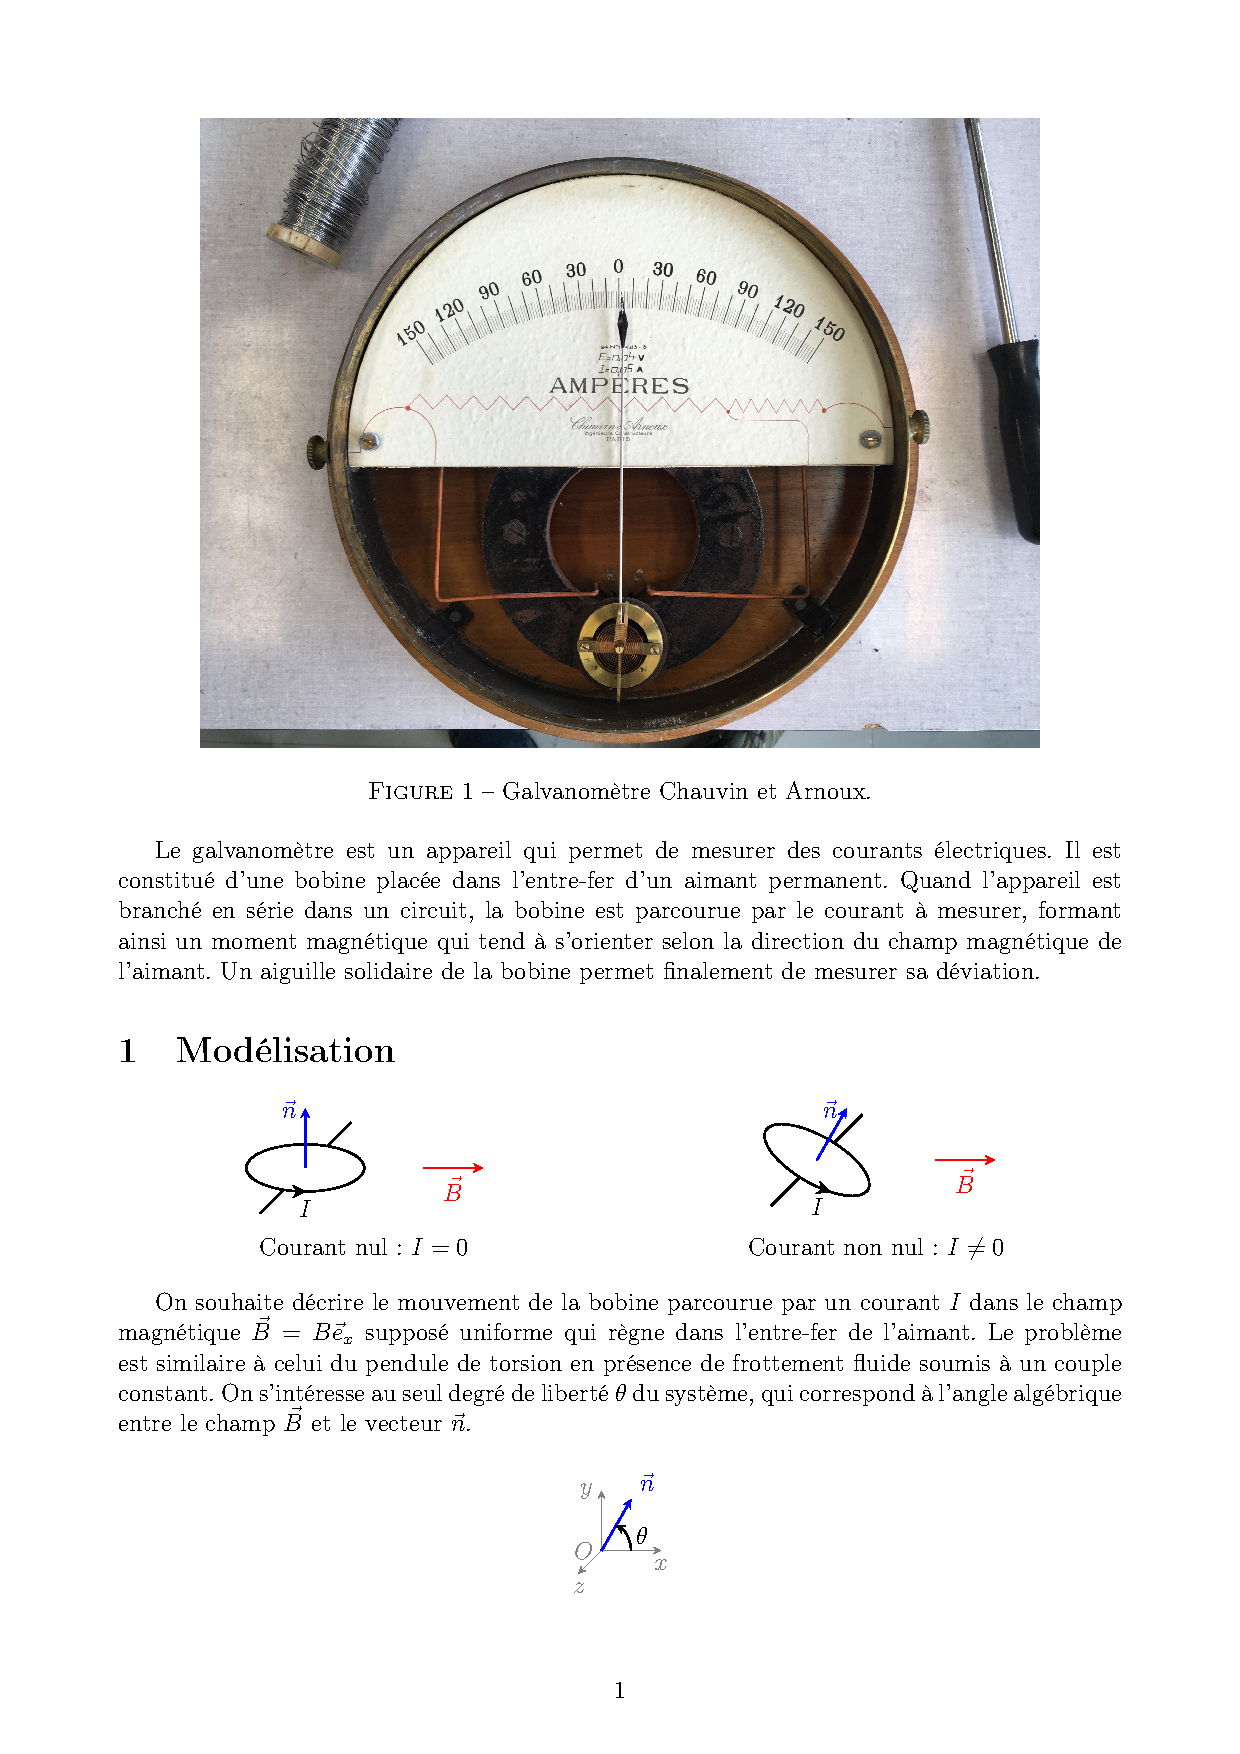
\includegraphics[scale=0.1]{galvanometre.jpg}
\caption{Galvanomètre Chauvin et Arnoux.}
\end{figure}

Le galvanomètre est un appareil qui permet de mesurer des courants électriques.
Il est constitué d'une bobine placée dans l'entre-fer d'un aimant permanent.
Quand l'appareil est branché en série dans un circuit, la bobine est parcourue par le courant à mesurer, formant ainsi un moment magnétique qui tend à s'orienter selon la direction du champ magnétique de l'aimant.
Un aiguille solidaire de la bobine permet finalement de mesurer sa déviation.

\section{Modélisation}

\begin{multicols}{2}
\begin{center}
\begin{tikzpicture}[scale=1]
\draw[thick] (0,0,-2) -- (0,0,2);
\filldraw[white] (0,0) ellipse (1 and .4);
\draw[thick] (0,0) ellipse (1 and .4);
\draw[ultra thick, decorate, decoration={markings,mark=at position 0.75 with{\arrow[black]{stealth}};}] (0,0) ellipse (1 and .4);
\draw (0, -.4) node[below] {$I$};

%\draw[decorate, decoration={markings,mark=at position -.4 with{\arrowreversed[black]{stealth}};}] (1,1) circle (1);

\draw[thick,->,>=stealth,blue] (0,0) --++ (0,1) node[left]{$\vec{n}$};

\coordinate (B) at (2,0);
\draw[red] (B) + (0.5,0) node[below]{$\vec{B}$};
\draw[thick,->,>=stealth,red] (B) --++ (1,0);
\end{tikzpicture}

Courant nul : $I=0$
\end{center}

\begin{center}
\begin{tikzpicture}[scale=1]
\draw[thick] (0,0,-2) -- (0,0,2);
\filldraw[white,rotate=-30] (0,0) ellipse (1 and .4);
\draw[thick,rotate=-30] (0,0) ellipse (1 and .4);
\draw[ultra thick,rotate=-30, decorate, decoration={markings,mark=at position 0.85 with{\arrow[black]{stealth}};}] (0,0) ellipse (1 and .4);
\draw (0, -.5) node[below] {$I$};

%\draw[decorate, decoration={markings,mark=at position -.4 with{\arrowreversed[black]{stealth}};}] (1,1) circle (1);

\draw[thick,->,>=stealth,blue] (0,0) --++ (60:1) node[left]{$\vec{n}$};

\coordinate (B) at (2,0);
\draw[red] (B) + (0.5,0) node[below]{$\vec{B}$};
\draw[thick,->,>=stealth,red] (B) --++ (1,0);
\end{tikzpicture}

Courant non nul : $I\neq0$
\end{center}
\end{multicols}

On souhaite décrire le mouvement de la bobine parcourue par un courant $I$ dans le champ magnétique $\vec{B}=B\vec{e}_x$ supposé uniforme qui règne dans l'entre-fer de l'aimant.
Le problème est similaire à celui du pendule de torsion en présence de frottement fluide soumis à un couple constant.
On s'intéresse au seul degré de liberté $\theta$ du système, qui correspond à l'angle algébrique entre le champ $\vec{B}$ et le vecteur $\vec{n}$.

\begin{center}
\begin{tikzpicture}[scale=1]
\coordinate (O) at (-0,0);
\draw[gray] (O) node [left] {$O$};
\draw [gray] [->,>=stealth] (O) --++(1,0,0) node [below] {$x$};
\draw [gray] [->,>=stealth] (O) --++(0,1,0) node [left] {$y$};
\draw [gray] [->,>=stealth] (O) --++(0,0,1) node [below] {$z$};

\draw[thick,->,>=stealth,blue] (O) --++ (60:1) node[above right]{$\vec{n}$};
\draw[thick,->,>=stealth] (O)+(.5,0) arc (0:60:.5);
\draw (O)+(30:.5) node[right]{$\theta$};
\end{tikzpicture}
\end{center}


\subsection{Système}

Le système étudié est l'ensemble \{bobine + aiguille\}.
La bobine est supposé plate, rectangulaire de côtés $a$ et $b$ délimitant une surface $S$ et formée de $N$ spires parcourue par un courant constant d'intensité $I$ dont l'orientation définie celle du vecteur $\vec{n}$ normal à la surface $S$.
On l'assimile à un moment magnétique $\vec{\mu} = NSI\vec{n}$.
L'ensemble bobine et aiguille possède par ailleurs un moment d'inertie $J$.

\subsection{Référentiel}

Le temps caractéristique de l'évolution du système est au plus de l'ordre de quelques secondes.
Le référentiel du laboratoire peut donc être considéré comme galiléen.

\subsection{Bilan des forces}

\begin{itemize}
\item Poids : au mieux, son moment est nul, mais au pire, il est négligé ;
\item $\vec{\Gamma}_B = \vec{\mu} \wedge \vec{B} = - \mu B \sin \theta \ez$ : moment subit par le moment magnétique $\vec{\mu}$ dans le champ $\vec{B}$ (moment des forces de Laplace) ;
\item $\vec{\Gamma}_H = -k(\theta-\pi/2)\ez$ : moment de la force de rappel du ressort spiral ;
\item $\vec{\Gamma}_f = -\alpha\dot{\theta}\ez$ : moment des forces de frottement fluide.
Les forces de frottement solide sont négligées pour le moment.
\end{itemize}

\subsection{Équation du mouvement}

Le moment cinétique de l'ensemble bobine et aiguille $\vec{L} = J\dot{\theta}\ez$ s'exprime en fonction du moment d'inertie $J$ du système.
On applique le théorème du moment cinétique :
\begin{equation}
\frac{\d\vec{L}}{\d t} 	= \vec{\Gamma}_B + \vec{\Gamma}_H + \vec{\Gamma}_f,
\end{equation}
et on le projette selon $\ez$ :
\begin{equation}
J\ddot{\theta} = -\mu B \sin \theta - k\left(\theta-\frac{\pi}{2}\right) - \alpha\dot{\theta}.
\label{eq:eq_mvt}
\end{equation}

Au voisinage de la position initiale, l'approximation des petits angles permet de linéariser l'équation du mouvement qui devient :
\begin{equation}
J\ddot{\theta} = -\mu B - k\left(\theta-\frac{\pi}{2}\right) - \alpha\dot{\theta}.
\label{eq:eq_mvt_lin}
\end{equation}

\section{Régime permanent}

On s'intéresse tout d'abord au régime permanent du système, \cad{} quand $\ddot{\theta}$ et $\dot{\theta}$ sont nuls.

\subsection{Très faibles déviations}

Dans ce cas, on utilise l'équation~\ref{eq:eq_mvt_lin} qui se simplifie et on trouve  l'expression de la position d'équilibre $\theta_\mathrm{eq}$ du système :
\begin{equation}
\theta_\mathrm{eq}^\mathrm{lin} = \frac{\pi}{2} - \frac{\mu B}{k},
\end{equation}
valable pour de faibles déviations, \cad{} tant que $\frac{\mu B}{k} \ll 1$

\subsection{DL à l'ordre 2}

Un développement limité de $\sin \theta$ autour de $\pi/2$ dans l'équation~\ref{eq:eq_mvt} en régime permanent donne :
\begin{equation}
0 = - \mu B \left[ 1-\frac{\left(\theta-\frac{\pi}{2}\right)^2}{2} \right] - k\left(\theta-\frac{\pi}{2}\right).
\end{equation}
La résolution de cette équation fait apparaitre deux solutions dont l'une diverge pour les petites valeurs de $\tfrac{\mu B}{k}$.
L'autre donne finalement :
\begin{equation}
\theta_\mathrm{eq}^\mathrm{DL2} = \frac{\pi}{2} + \frac{1-\sqrt{1+2\left(\frac{\mu B}{k}\right)^2}}{\frac{\mu B}{k}}.
\label{eq:sol_2nd}
\end{equation}

\noindent
\textbf{Remarque :}
Lorsque $\frac{\mu B}{k} \ll 1$, on peut linéariser cette solution et on retrouve la position d'équilibre précédente, obtenue dans le cas de très faibles déviations.

\subsection{Solution numérique}

L'équation~\ref{eq:eq_mvt} en régime permanent s'écrit :
\begin{equation}
0 = -\mu B \sin \theta - k\left(\theta-\frac{\pi}{2}\right),
\end{equation}
et n'admet pas de solution analytique\footnote{À ce que je sache.}.
Il est toutefois possible de la résoudre numériquement pour obtenir $\theta_\mathrm{eq}^\mathrm{num}$.

\subsection{Linéarité de l'affichage}

\begin{figure}
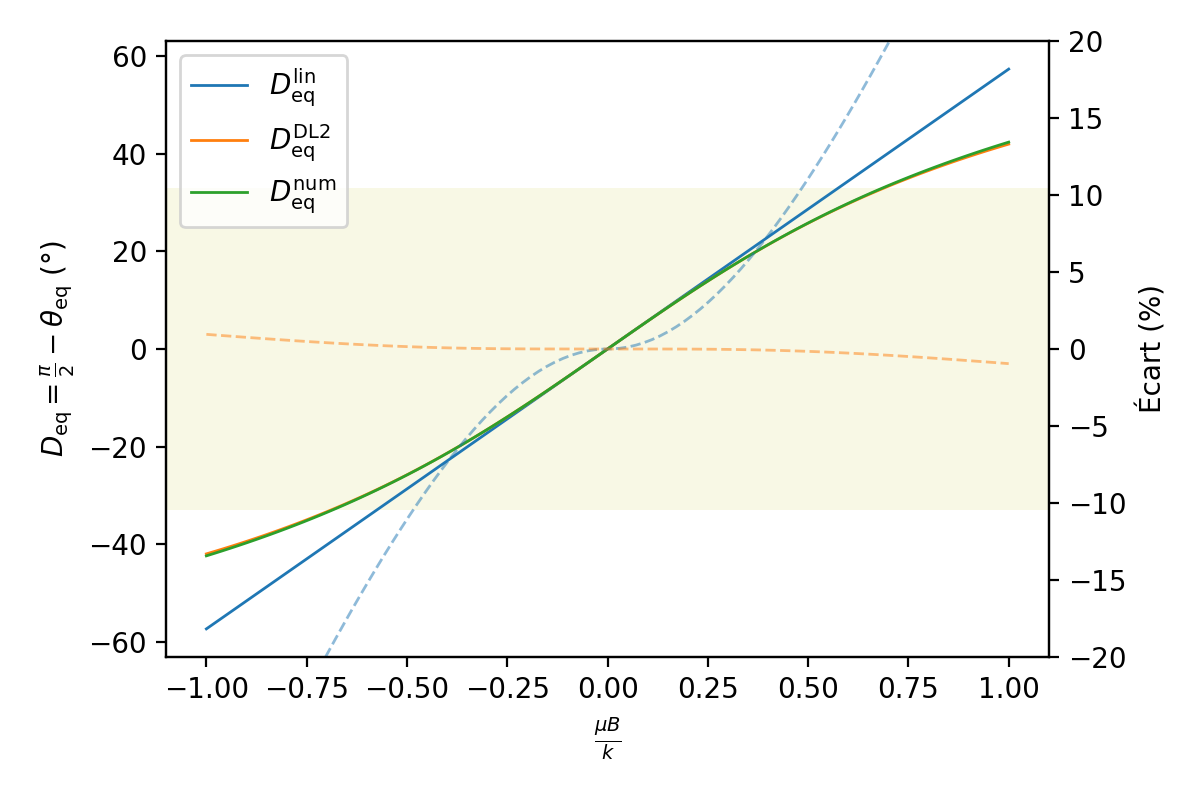
\includegraphics[scale=1]{deviation.png}
\caption{Déviation de l'aiguille du galvanomètre en fonction du rapport $\tfrac{\mu B}{k}$ proportionnel au courant mesuré.
Les trois courbes pleines représentent les déviations associées aux trois solutions obtenues précédemment dans le cadre de l'approximation linéaire, du développement limité au second ordre et de la résolution numérique.
Les courbes en pointillés montrent l'écart relatif entre les déviations calculées analytiquement (linéaire et DL 2\textsuperscript{nd} ordre) et le calcul numérique.
La plage de déviation matérialisée en jaune pâle représente la gamme de valeurs effectivement mesurables par l'instrument compte tenu de l'amplitude de mouvement de l'aiguille.}
\label{fig:deviation}
\end{figure}

La comparaison des solutions obtenues avec différentes approximations (Fig.~\ref{fig:deviation}) montre que la solution analytique $\theta_\mathrm{eq}^\mathrm{DL2}$ obtenue en faisant un développement limité à l'ordre 2 (Éq.~\ref{eq:sol_2nd}) permet d'obtenir une excellente approximation de la position d'équilibre du système sur la plage de mesure accessible à l'instrument.
En effet, l'écart relatif avec la valeur calculée numériquement reste inférieur à \unit{0{,}4}{\%} sur l'ensemble de la plage de mesure.

L'approximation linéaire donne un écart relatif inférieur à \unit{1}{\%} pour des déviations inférieures à \unit{8}{\degree} mais proche de \unit{20}{\%} au maximum de déviation.

\end{document}